% Options for packages loaded elsewhere
\PassOptionsToPackage{unicode}{hyperref}
\PassOptionsToPackage{hyphens}{url}
\documentclass[
  english,
  11pt,
  a4paper,
]{article}
\usepackage{xcolor}
\usepackage[margin=22mm,headheight=15pt]{geometry}
\usepackage{amsmath,amssymb}
\setcounter{secnumdepth}{-\maxdimen} % remove section numbering
\usepackage{iftex}
\ifPDFTeX
  \usepackage[T1]{fontenc}
  \usepackage[utf8]{inputenc}
  \usepackage{textcomp} % provide euro and other symbols
\else % if luatex or xetex
  \usepackage{unicode-math} % this also loads fontspec
  \defaultfontfeatures{Scale=MatchLowercase}
  \defaultfontfeatures[\rmfamily]{Ligatures=TeX,Scale=1}
\fi
\usepackage{lmodern}
\ifPDFTeX\else
  % xetex/luatex font selection
\fi
% Use upquote if available, for straight quotes in verbatim environments
\IfFileExists{upquote.sty}{\usepackage{upquote}}{}
\IfFileExists{microtype.sty}{% use microtype if available
  \usepackage[]{microtype}
  \UseMicrotypeSet[protrusion]{basicmath} % disable protrusion for tt fonts
}{}
\makeatletter
\@ifundefined{KOMAClassName}{% if non-KOMA class
  \IfFileExists{parskip.sty}{%
    \usepackage{parskip}
  }{% else
    \setlength{\parindent}{0pt}
    \setlength{\parskip}{6pt plus 2pt minus 1pt}}
}{% if KOMA class
  \KOMAoptions{parskip=half}}
\makeatother
\usepackage{longtable,booktabs,array}
\usepackage{caption}
\captionsetup[table]{skip=6pt}
\newcounter{none} % for unnumbered tables
\usepackage{calc} % for calculating minipage widths
% Correct order of tables after \paragraph or \subparagraph
\usepackage{etoolbox}
\makeatletter
\patchcmd\longtable{\par}{\if@noskipsec\mbox{}\fi\par}{}{}
\makeatother
% Allow footnotes in longtable head/foot
\IfFileExists{footnotehyper.sty}{\usepackage{footnotehyper}}{\usepackage{footnote}}
\makesavenoteenv{longtable}
\usepackage{graphicx}
\makeatletter
\newsavebox\pandoc@box
\newcommand*\pandocbounded[1]{% scales image to fit in text height/width
  \sbox\pandoc@box{#1}%
  \Gscale@div\@tempa{\textheight}{\dimexpr\ht\pandoc@box+\dp\pandoc@box\relax}%
  \Gscale@div\@tempb{\linewidth}{\wd\pandoc@box}%
  \ifdim\@tempb\p@<\@tempa\p@\let\@tempa\@tempb\fi% select the smaller of both
  \ifdim\@tempa\p@<\p@\scalebox{\@tempa}{\usebox\pandoc@box}%
  \else\usebox{\pandoc@box}%
  \fi%
}
% Set default figure placement to htbp
\def\fps@figure{htbp}
\makeatother
\ifLuaTeX
\usepackage[bidi=basic,shorthands=off]{babel}
\else
\usepackage[bidi=default,shorthands=off]{babel}
\fi
\ifLuaTeX
  \usepackage{selnolig} % disable illegal ligatures
\fi
\setlength{\emergencystretch}{3em} % prevent overfull lines
\providecommand{\tightlist}{%
  \setlength{\itemsep}{0pt}\setlength{\parskip}{0pt}}
% Residual connection notes; style adapted from Attention/CN/pdf-header.tex.
\usepackage{fontspec}
\usepackage{enumitem}
\usepackage{fancyhdr}
\usepackage{fvextra}
\usepackage{etoolbox}
\usepackage{pdflscape}

\setmainfont[
  Path=/usr/local/texlive/2026/texmf-dist/fonts/opentype/public/tex-gyre/,
  UprightFont=texgyrepagella-regular.otf,
  BoldFont=texgyrepagella-bold.otf,
  ItalicFont=texgyrepagella-italic.otf,
  BoldItalicFont=texgyrepagella-bolditalic.otf
]{texgyrepagella-regular.otf}
\setsansfont[
  Path=/usr/local/texlive/2026/texmf-dist/fonts/opentype/public/tex-gyre/,
  UprightFont=texgyreheros-regular.otf,
  BoldFont=texgyreheros-bold.otf,
  ItalicFont=texgyreheros-italic.otf,
  BoldItalicFont=texgyreheros-bolditalic.otf
]{texgyreheros-regular.otf}
\setmonofont[
  Path=/usr/local/texlive/2026/texmf-dist/fonts/opentype/google/roboto/,
  UprightFont=RobotoMono-Regular.otf,
  BoldFont=RobotoMono-Bold.otf,
  ItalicFont=RobotoMono-Italic.otf,
  BoldItalicFont=RobotoMono-BoldItalic.otf,
  Scale=0.82
]{RobotoMono-Regular.otf}
\definecolor{attentionblue}{HTML}{174A7E}
\definecolor{attentiongray}{HTML}{5D6773}
\definecolor{attentionlink}{HTML}{1769AA}
\definecolor{codebg}{HTML}{F4F6F8}

\AtBeginDocument{%
  \hypersetup{
    linkcolor=attentionblue,
    urlcolor=attentionlink,
    citecolor=attentionblue,
    pdftitle={Beyond Residual Connection}
  }%
}

\usepackage{titlesec}
\titleformat{\section}
  {\LARGE\bfseries\sffamily\color{attentionblue}}{}{0pt}{}
\titleformat{\subsection}
  {\Large\bfseries\sffamily\color{attentionblue}}{}{0pt}{}
\titleformat{\subsubsection}
  {\large\bfseries\sffamily\color{attentiongray}}{}{0pt}{}
\titlespacing*{\section}{0pt}{1.8ex}{1.2ex}
\titlespacing*{\subsection}{0pt}{1.6ex}{0.9ex}
\titlespacing*{\subsubsection}{0pt}{1.4ex}{0.7ex}

\setlength{\parindent}{2em}
\setlength{\parskip}{0.35em}
\linespread{1.18}
\setlist{itemsep=0.25em,topsep=0.45em,leftmargin=2.4em}
\setcounter{tocdepth}{2}
\setcounter{secnumdepth}{0}

\pagestyle{fancy}
\fancyhf{}
\fancyhead[L]{\small\sffamily\color{attentiongray} Residual Connections}
\fancyhead[R]{\small\sffamily\color{attentiongray} Purshow’ Notes}
\fancyfoot[C]{\small\sffamily\thepage}
\renewcommand{\headrulewidth}{0.3pt}


\usepackage{caption}
\captionsetup{font=small,labelfont=bf}
\clearcaptionsetup{table} % Overview has no caption; clear Pandoc defaults.
\usepackage{float}
\floatplacement{figure}{H}
\AtBeginDocument{\renewcommand{\figurename}{Figure}}

% A single opening page: article title above an automatically linked contents.
\makeatletter
\renewcommand*\l@subsection{\@dottedtocline{2}{0em}{0em}}
\renewcommand*\l@subsubsection{\@dottedtocline{3}{1.6em}{0em}}
\makeatother
\newcommand{\NotesCover}[1]{%
  \pagenumbering{roman}%
  \thispagestyle{empty}%
  \vspace*{0mm}%
  {\centering
    \sffamily\bfseries\color{attentionblue}%
    \fontsize{26pt}{36pt}\selectfont #1\par
  }%
  \vspace{4mm}%
  {\color{attentionblue}\noindent\rule{\linewidth}{0.6pt}\par}%
  \vspace{4mm}%
  \begingroup
    \setlength{\parindent}{0pt}%
    \setlength{\parskip}{0.6em}%
    \tableofcontents
  \endgroup
}
\newcommand{\NotesCoverEnd}{%
  \clearpage
  \pagenumbering{arabic}%
}

% Compact wrapping overview table, following Attention and MoE notes.
\newcommand{\OverviewTableStyle}{%
  \fontsize{7.5pt}{8.8pt}\selectfont
  \setlength{\tabcolsep}{4pt}%
  \renewcommand{\arraystretch}{1.2}%
  \setlength{\extrarowheight}{6pt}%
  \setlength{\LTpre}{30pt}%
  \setlength{\LTpost}{0pt}%
  \setlength{\parskip}{0pt}%
}
\usepackage{bookmark}
\IfFileExists{xurl.sty}{\usepackage{xurl}}{} % add URL line breaks if available
\urlstyle{same}
% fallback for those not using the hyperref driver hyperxmp:
\makeatletter
\@ifundefined{xmpquote}{\newcommand{\xmpquote}[1]{#1}}{}
\makeatother
\hypersetup{
  pdflang={en},
  hidelinks,
  pdfcreator={LaTeX via pandoc}}

\author{}
\date{}

\begin{document}

\NotesCover{Beyond Residual Connection}

\begingroup\OverviewTableStyle

{\def\LTcaptype{none} % do not increment counter
\begin{longtable}[]{@{}
  >{\raggedright\arraybackslash}p{(\linewidth - 8\tabcolsep) * \real{0.1400}}
  >{\raggedright\arraybackslash}p{(\linewidth - 8\tabcolsep) * \real{0.2300}}
  >{\raggedright\arraybackslash}p{(\linewidth - 8\tabcolsep) * \real{0.2400}}
  >{\raggedright\arraybackslash}p{(\linewidth - 8\tabcolsep) * \real{0.2000}}
  >{\raggedright\arraybackslash}p{(\linewidth - 8\tabcolsep) * \real{0.1900}}@{}}
\toprule\noalign{}
\begin{minipage}[b]{\linewidth}\raggedright
Type
\end{minipage} & \begin{minipage}[b]{\linewidth}\raggedright
Simplified Structure
\end{minipage} & \begin{minipage}[b]{\linewidth}\raggedright
Core Idea
\end{minipage} & \begin{minipage}[b]{\linewidth}\raggedright
Dynamics / Constraints
\end{minipage} & \begin{minipage}[b]{\linewidth}\raggedright
Representative Models
\end{minipage} \\
\midrule\noalign{}
\endhead
\bottomrule\noalign{}
\endlastfoot
\textbf{PreNorm} & \(x'=x+F(\mathrm{Norm}(x))\) & One residual stream; a
fixed identity shortcut accumulates layer outputs & Fixed identity; no
learned residual mixing & Most models other than those listed below \\
\textbf{HC} &
\(\begin{aligned}R'&=H_{\mathrm{res}}\cdot R\\&\quad+H_{\mathrm{post}}\cdot F(H_{\mathrm{pre}}\cdot R)\end{aligned}\)
& Expands one residual stream into several; learns Read, Write, and
residual mixing & \(H_{\mathrm{res}}\) is learned and data-dependent;
flexible, but deep training can be unstable & HC \\
\textbf{mHC} &
\(H'_{\mathrm{res}}=\operatorname{Sinkhorn\text{-}Knopp}(H_{\mathrm{res}})\)
& Constrains HC residual mixing to keep multiple residual streams stable
in deep networks & \textbf{Doubly stochastic matrices address HC's
instability at depth} & DeepSeek-V4-Pro, DeepSeek-V4.1-Flash \\
\textbf{iHC} & \(H_{\mathrm{res}}=I\) & \textbf{Replaces mHC's doubly
stochastic matrix with the identity}, retaining Read / Write across
multiple residual streams & \(H_{\mathrm{res}}=I\); fixed identity
residual mixing & HY4-Preview \\
\textbf{GR} & \(H_{\mathrm{res}}=I\) + channel-level Read &
\textbf{Channel-level Read}; gates dynamically control what a sublayer
reads from the residual stream & \(H_{\mathrm{res}}=I\);
\textbf{element-wise, data-dependent read gates} & Qwen3.8-Flash-Next \\
\textbf{AttnRes} & \(h_l=\sum_i\alpha_{i\to l}\cdot v_i\),
\(\alpha=\mathrm{softmax}(q_l\cdot k_i)\) & Replaces fixed residual
accumulation with attention over earlier layers / blocks, selecting
information for the current layer & Softmax weighting along depth; K3
uses Block AttnRes to reduce overhead & Kimi K3 \\
\end{longtable}
}

\endgroup\NotesCoverEnd

Residual connections deserve to be called the milestone that put the
``deep'' in deep learning. In recent years, after tinkering with just
about every part of the Transformer, people have finally sharpened their
knives for the residual connections too.

\subsection{1. Starting with Pre-Norm and
Post-Norm}\label{starting-with-pre-norm-and-post-norm}

It all starts with the Pre-Norm versus Post-Norm debate. Put simply:

\begin{figure}
\centering
\pandocbounded{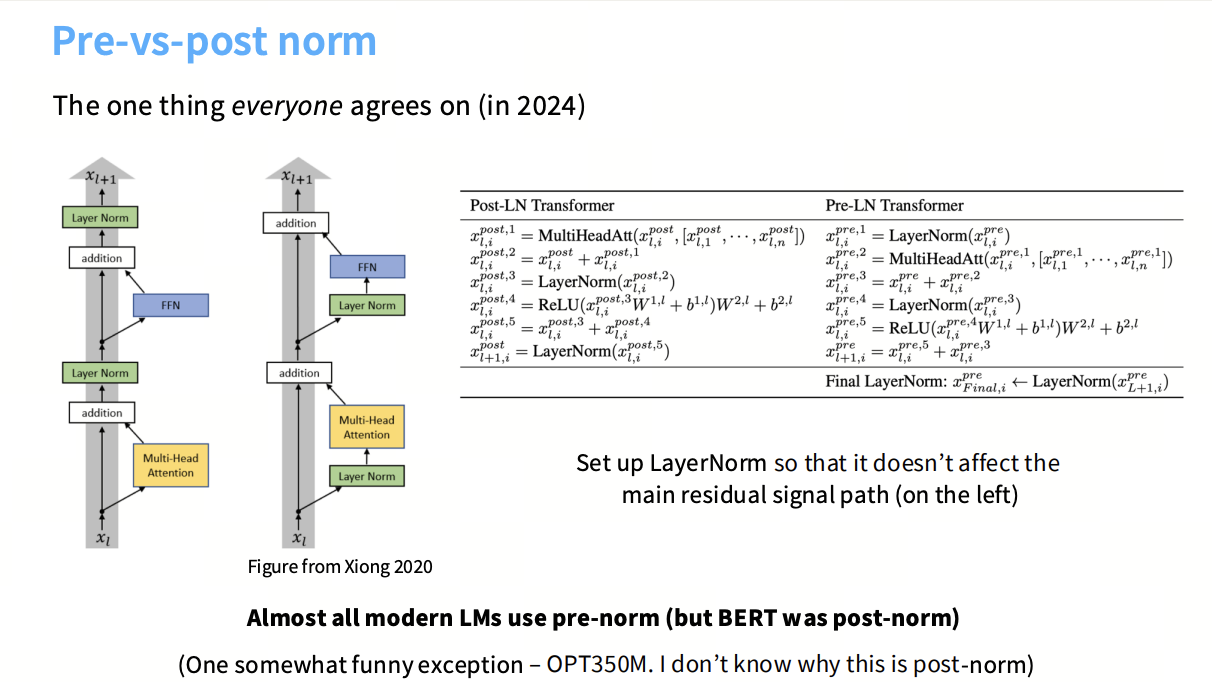
\includegraphics[keepaspectratio,alt={Pre-Norm and Post-Norm architectures}]{assets/prenorm-postnorm.png}}
\caption{Pre-Norm and Post-Norm architectures}
\end{figure}

\textbf{Pre-Norm}: normalize before each residual branch. Apply Norm
first, then pass the result to a sublayer such as Attention or an FFN.

\textbf{Post-Norm}: normalize after the residual connection. Compute the
sublayer output, add the residual, and then apply Norm.

Most large language models today use \textbf{Pre-Norm}. One major reason
is that it gives the residual backbone a more direct path for gradient
propagation, making deep Transformers more stable to train. It helps
mitigate vanishing or exploding gradients, making it easier to scale to
dozens or even hundreds of layers.

Pre-Norm has limitations, though. Its residual update can be written
approximately as:

\[
x_{l+1}=x_l+F\!\left(\mathrm{Norm}(x_l)\right).
\]

As the network gets deeper, its representation keeps accumulating
residual information from earlier layers. The increment introduced by
any later layer may become progressively smaller relative to the
accumulated backbone representation, so the change between adjacent deep
layers gradually weakens.

In other words, adding more physical layers does not guarantee that each
new layer contributes an equally meaningful transformation. The
network's effective depth may be lower than its nominal depth.

As kexue.fm put it, \textbf{Pre-Norm, in a sense, ``increases the
model's width while reducing its depth.''}

Pre-Norm and Post-Norm therefore embody a trade-off:

\textbf{Pre-Norm is easier to optimize and more stable to train, but may
sacrifice some of the representational power that depth provides;
Post-Norm can, in principle, preserve stronger transformations from
layer to layer, but makes deep networks harder to optimize.}

A whole line of papers has tried to resolve this. To me, one of the best
directions is Hyper-Connections.

\subsection{2. HC}\label{hc}

\begin{figure}
\centering
\pandocbounded{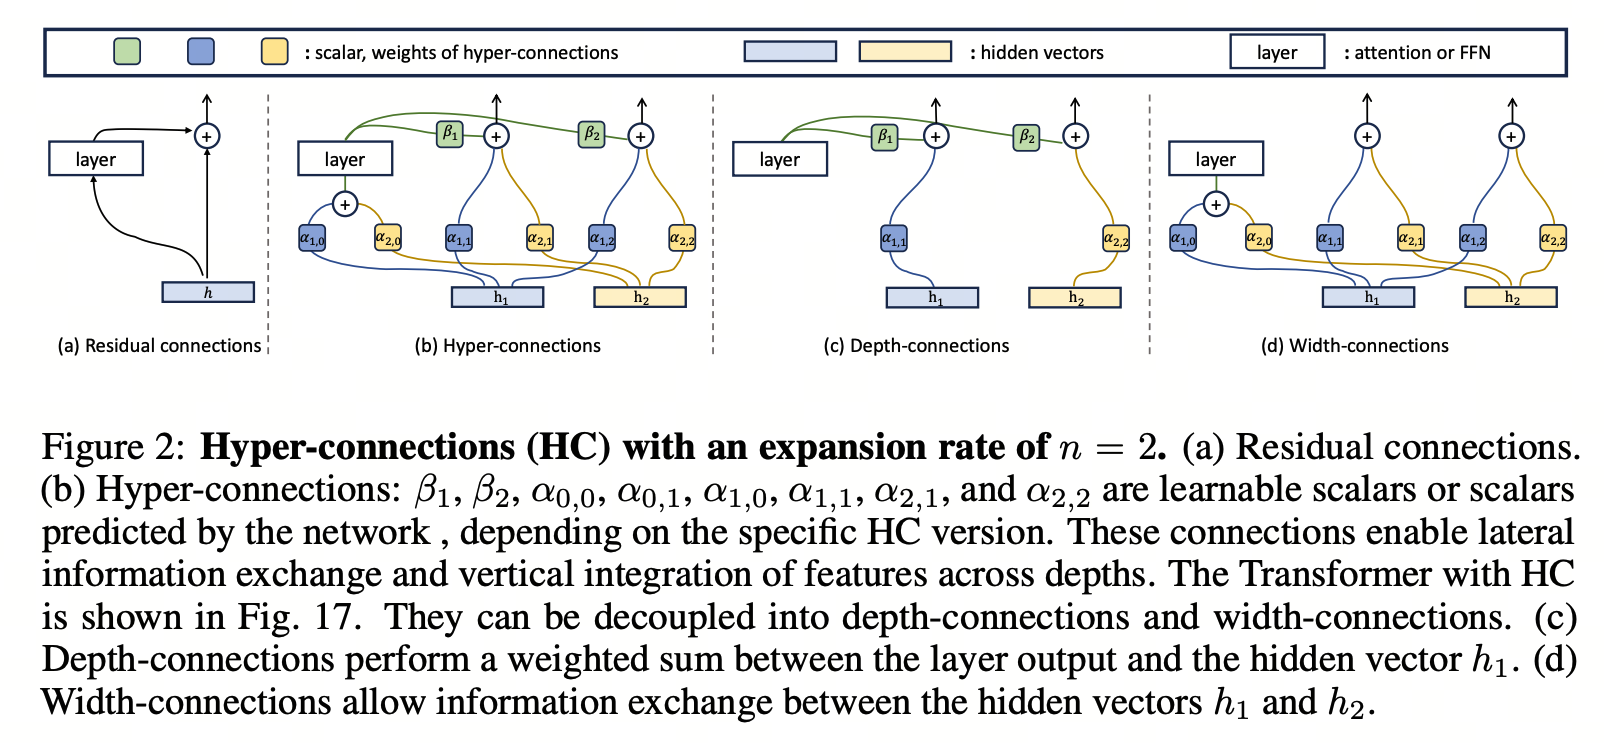
\includegraphics[keepaspectratio,alt={HC's multiple-stream architecture}]{assets/hc-architecture.png}}
\caption{HC's multiple-stream architecture}
\end{figure}

\begin{figure}
\centering
\pandocbounded{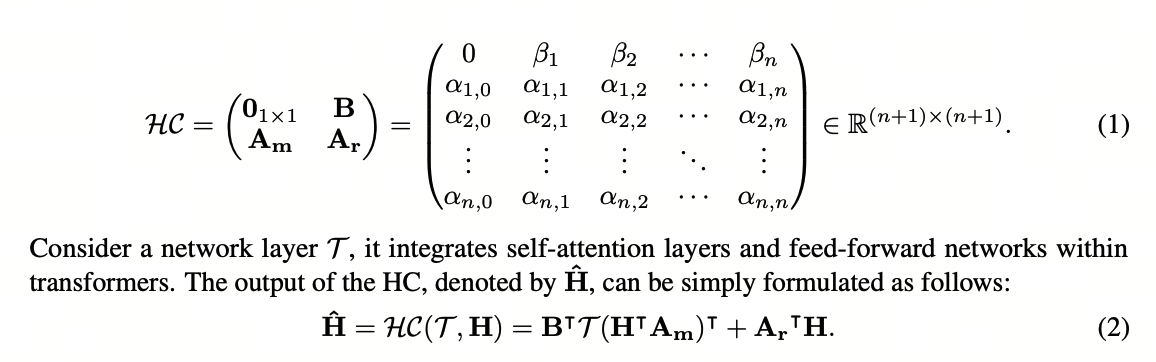
\includegraphics[keepaspectratio,alt={Reading, writing, and residual mixing in HC}]{assets/hc-equations.png}}
\caption{Reading, writing, and residual mixing in HC}
\end{figure}

HC works roughly like this: \textbf{first replicate the original hidden
state into \(n\) parallel hidden streams. At each layer, use \(A_m\) to
mix these \(n\) streams into one weighted input for a normal Attention
or FFN sublayer, computed only once. Then use \(B\) to write the new
layer output back to the \(n\) streams with different weights, while
\(A_r\) preserves and mixes the existing streams along the residual
path. The resulting \(n\) hidden states continue to the next layer. In
effect, a fixed residual connection becomes a learned routing mechanism
across multiple streams.}

Put plainly: maintain \(n\) streams, then decide which ones this layer
reads from, which ones it writes its output to, and how the old
information moves forward.

Section 4.5 of the paper also has some excellent visualizations and
analysis. Maybe HC started the trend: its successors keep doing similar
visualizations, which is a great habit! I strongly recommend reading the
original paper.

Here are a few takeaways:

\begin{figure}
\centering
\pandocbounded{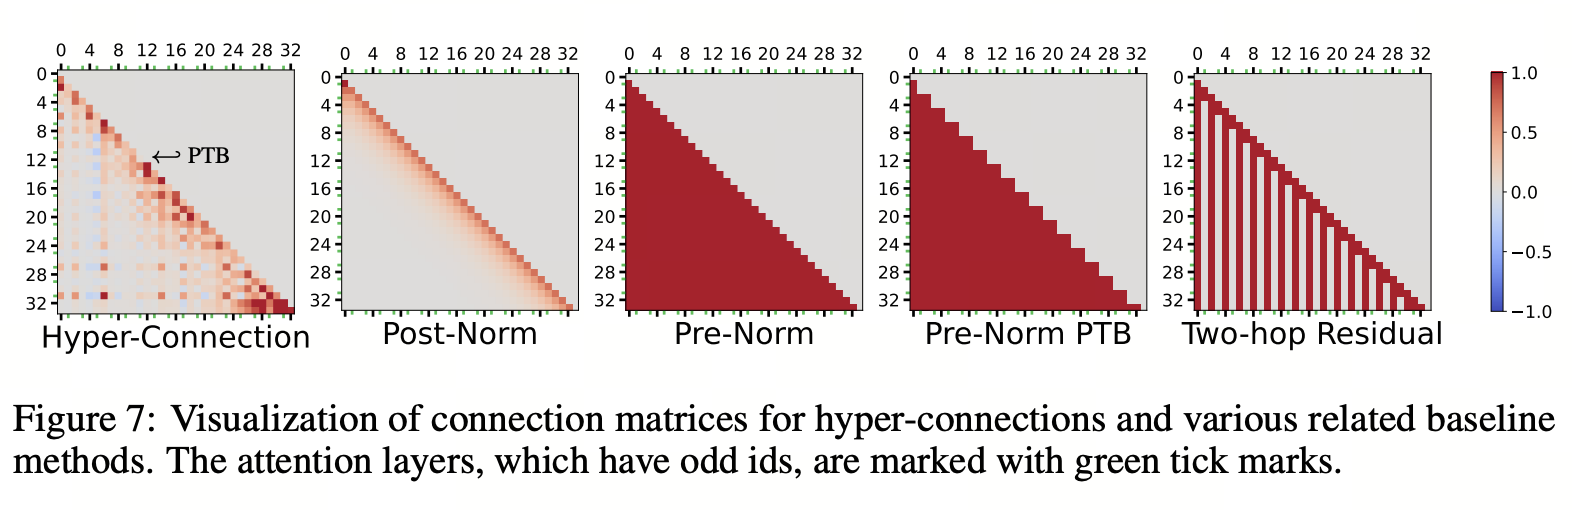
\includegraphics[keepaspectratio,alt={Visualization of HC's effective connection matrix}]{assets/hc-connectivity.png}}
\caption{Visualization of HC's effective connection matrix}
\end{figure}

\begin{itemize}
\item
  The unrolled effective connection matrix shows that HC learns both:

  \begin{itemize}
  \item
    \textbf{Strong local connections}: greater dependence on recent
    layers, similar to Post-Norm.
  \item
    \textbf{A few direct long-range connections}: retention of important
    early-layer information, similar to Pre-Norm.
  \end{itemize}
\item
  Together, these give us \textbf{short-range updates for most
  information, with long-term retention of a few important pieces}.
\item
  Connections between some adjacent layers are close to zero. This
  suggests that the model spontaneously forms something like
  \textbf{Parallel Transformer Blocks, where Attention and the FFN run
  in parallel; see the zigzag pattern in the figure.}
\item
  Attention outputs tend to be used locally, while FFN outputs more
  readily form long-range connections.
\item
  With \(n=1\), it is hard to achieve both ``local updates'' and
  ``long-term retention.'' With \(n>1\), different streams can take on
  these two roles.
\end{itemize}

\subsection{3. mHC}\label{mhc}

\begin{figure}
\centering
\pandocbounded{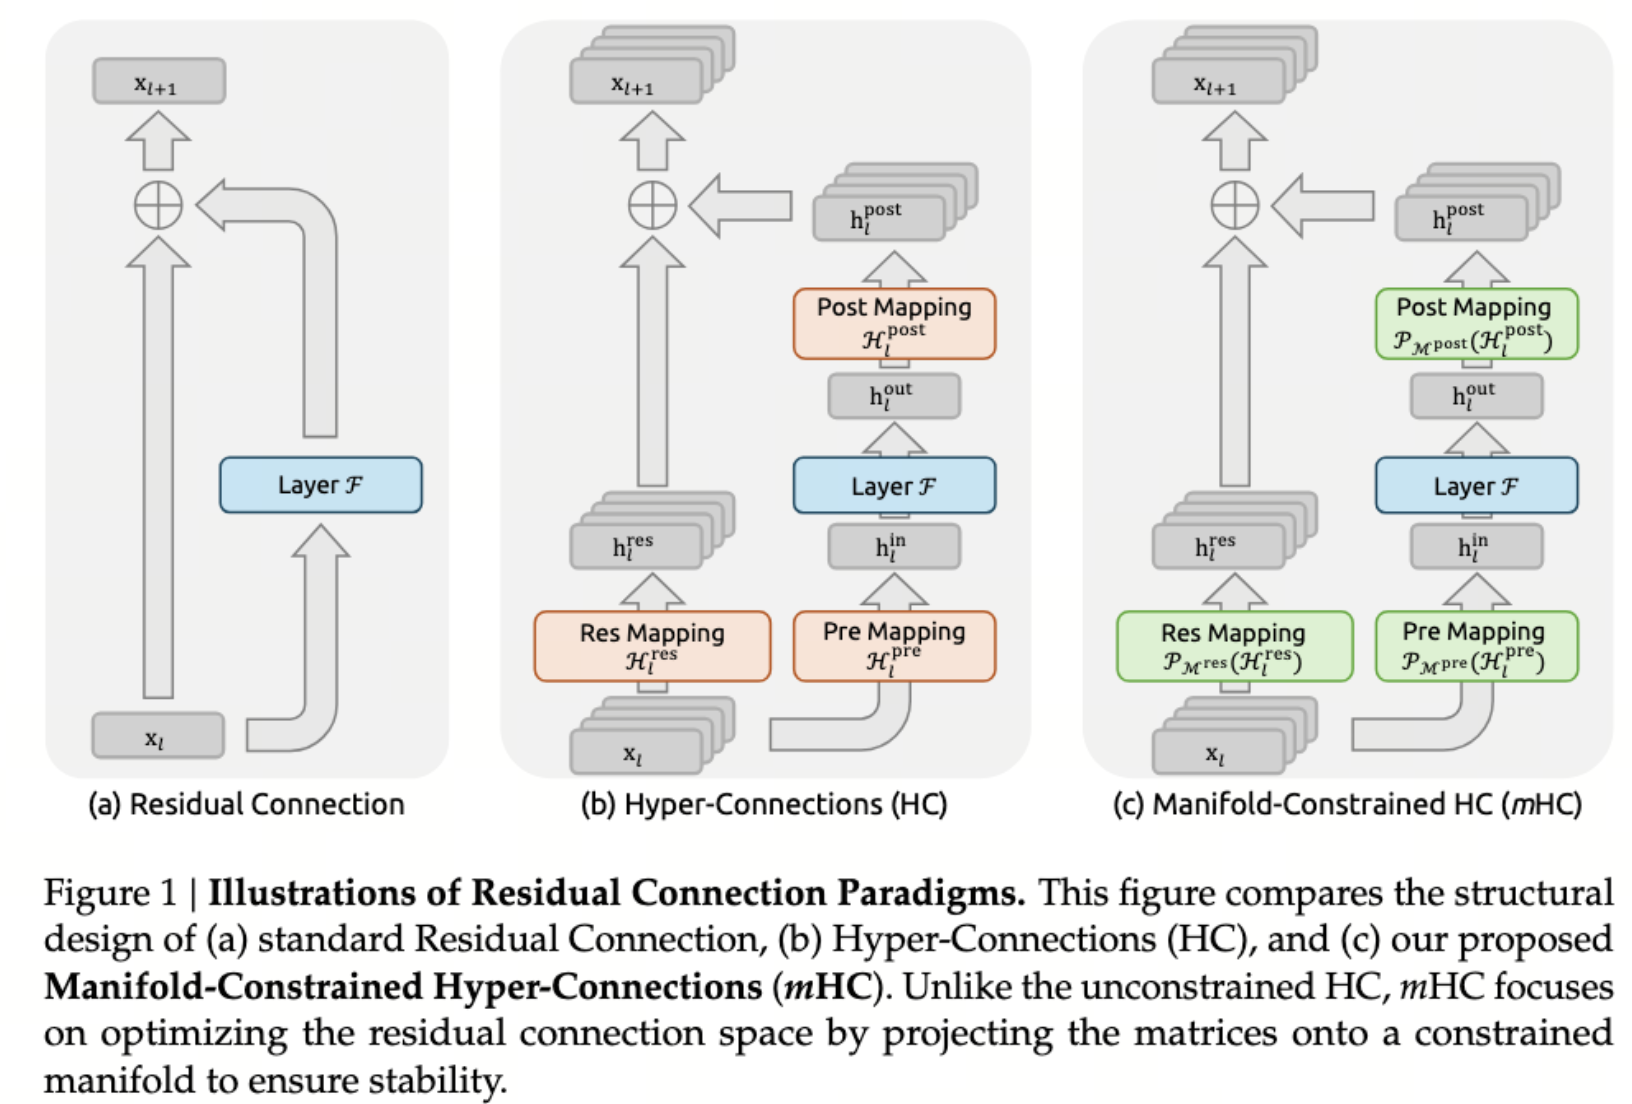
\includegraphics[keepaspectratio,alt={mHC architecture and constraints}]{assets/mhc.png}}
\caption{mHC architecture and constraints}
\end{figure}

Unroll a multilayer HC network, and a signal from an early layer has to
pass through:

\[
\prod_{i=1}^{L-l}\mathcal{H}_{L-i}^{\mathrm{res}}
\]

to reach layer \(L\). The full expression is:

\[
\mathbf{x}_L=
\left(
\prod_{i=1}^{L-l}\mathcal{H}_{L-i}^{\mathrm{res}}
\right)\mathbf{x}_l
+
\sum_{i=l}^{L-1}
\left(
\prod_{j=1}^{L-1-i}\mathcal{H}_{L-j}^{\mathrm{res}}
\right)
\mathcal{H}_i^{\mathrm{post}\top}
\mathcal{F}
\left(
\mathcal{H}_i^{\mathrm{pre}}\mathbf{x}_i,\mathcal{W}_i
\right).
\]

In a traditional ResNet, the corresponding first term is simply
\(I\mathbf{x}_l\). HC replaces it with a long product of unconstrained
matrices. If those matrices have directions that amplify by more than 1
or contract by less than 1, then after dozens of layers:

\[
\left\|
\prod_l \mathcal{H}_l^{\mathrm{res}}
\right\|
\]

can blow up through repeated multiplication.

mHC addresses this using doubly stochastic matrices, meaning:

\begin{enumerate}
\def\labelenumi{\arabic{enumi}.}
\item
  Every entry is nonnegative: \(H_{ij}\ge 0\).
\item
  Every row sums to \(1\).
\item
  Every column sums to \(1\).
\end{enumerate}

Doubly stochastic matrices have several particularly nice properties,
including those highlighted in the paper:

\begin{enumerate}
\def\labelenumi{\arabic{enumi}.}
\item
  Norm Preservation: their spectral norm is bounded by 1, which helps
  mitigate exploding gradients.
\item
  Compositional Closure: these nice properties are preserved under
  matrix multiplication! Even after composition across many layers, the
  overall residual mapping remains doubly stochastic.
\item
  Geometric Interpretation via the Birkhoff Polytope: I'll leave this
  one to the original paper =.=.
\end{enumerate}

The core of mHC is to turn HC's most unstable component, the
residual-stream mixing matrix \(H_l^{\mathrm{res}}\), from an arbitrary
learned matrix into a \textbf{doubly stochastic matrix}. The input first
dynamically generates \(\tilde{H}_l^{\mathrm{res}}\); Sinkhorn-Knopp
then repeatedly normalizes its rows and columns so that
\(H_l^{\mathrm{res}}\ge 0\) and each row and column sums to
approximately 1. Meanwhile,
\(H_l^{\mathrm{pre}}=\sigma(\tilde{H}_l^{\mathrm{pre}})\) and
\(H_l^{\mathrm{post}}=2\sigma(\tilde{H}_l^{\mathrm{post}})\) keep the
read and write coefficients positive. The \(n\) residual streams can
still exchange information dynamically, while the bound \(\|H\|_2\le 1\)
and closure under multiplication keep \(\prod_l H_l^{\mathrm{res}}\)
from developing extreme gain across many layers. With \(n=4\) and 20
Sinkhorn iterations, the paper reports that composite gain in the 27B
model falls from nearly 3000 for HC to about 1.6 for mHC.

\textbf{On the infra side,} the real bottleneck in HC/mHC is memory
access, activation storage, and pipeline communication after expanding
the residual state to \(nC\), rather than FLOPs. The authors therefore
combine three kinds of optimization:

First, \textbf{kernel fusion + mixed precision} for RMSNorm, dynamic
generation of \(H^{\mathrm{pre/post/res}}\), Sinkhorn, and residual
merging. In particular, fusing the application of \(H^{\mathrm{post}}\)
and \(H^{\mathrm{res}}\) with the residual merge reduces reads in this
part from \((3n+1)C\) to \((n+1)C\), and writes from \(3nC\) to \(nC\).

Second, \textbf{selective recomputation}: instead of retaining every
intermediate mHC activation, save \(x_{l_0}\) at block boundaries and
recompute only the inexpensive mHC operations during the backward pass.
The paper derives an approximately optimal recomputation interval of
\(L_r^*\approx\sqrt{nL/(n+2)}\).

Third, overlap communication and computation in DualPipe, placing some
residual kernels on high-priority streams to reduce pipeline stalls from
the \(n\)-fold residual communication. The authors ultimately report
about 6.7\% additional training time for large models with \(n=4\).

But mHC only guards against explosion; it does not guarantee that
information will not be lost or even collapse.

\clearpage

\begingroup
\linespread{1.0}\selectfont

\subsection{4. iHC}\label{ihc}

Let's take a closer look at iHC.

Honestly, iHC feels very natural to me. When I first saw HC, this was my
immediate reaction: if multiplying these matrices can cause an
explosion, why not just use the identity matrix and let each stream go
its own way?

\begin{figure}
\centering
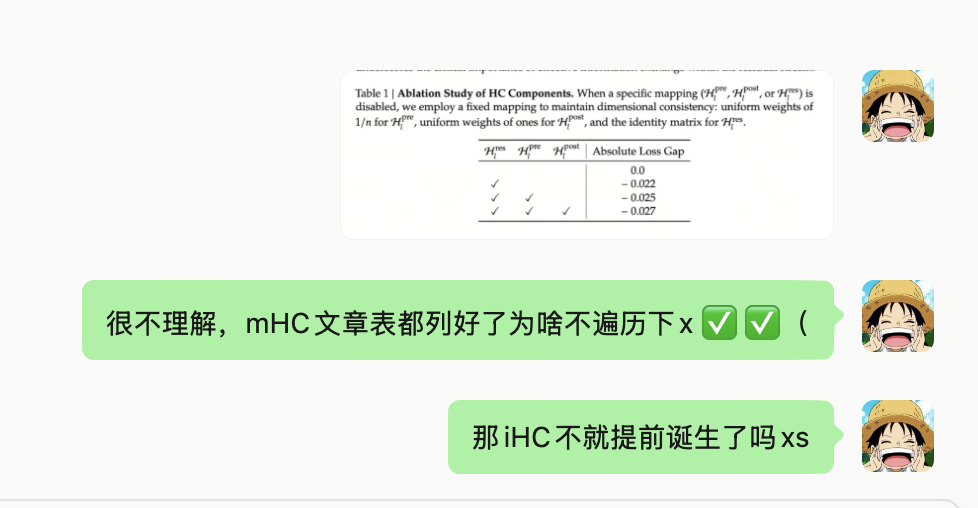
\includegraphics[width=0.48\linewidth,height=\textheight,keepaspectratio,alt={What puzzles me is that the table in the mHC paper seems to put iHC within reach of a simple sweep. I do not quite understand why this experiment was skipped. Surely they did not just forget?}]{assets/ihc-discussion.png}
\caption{What puzzles me is that the table in the mHC paper seems to put
iHC within reach of a simple sweep. I do not quite understand why this
experiment was skipped. Surely they did not just forget?}
\end{figure}

The chat in the screenshot says: ``I don't get it: mHC already lays out
the table, so why not sweep through the combinations?'' and ``Wouldn't
iHC have emerged earlier that way? lol.''

iHC author Tian Xie makes a particularly interesting observation here:

\noindent\hfill
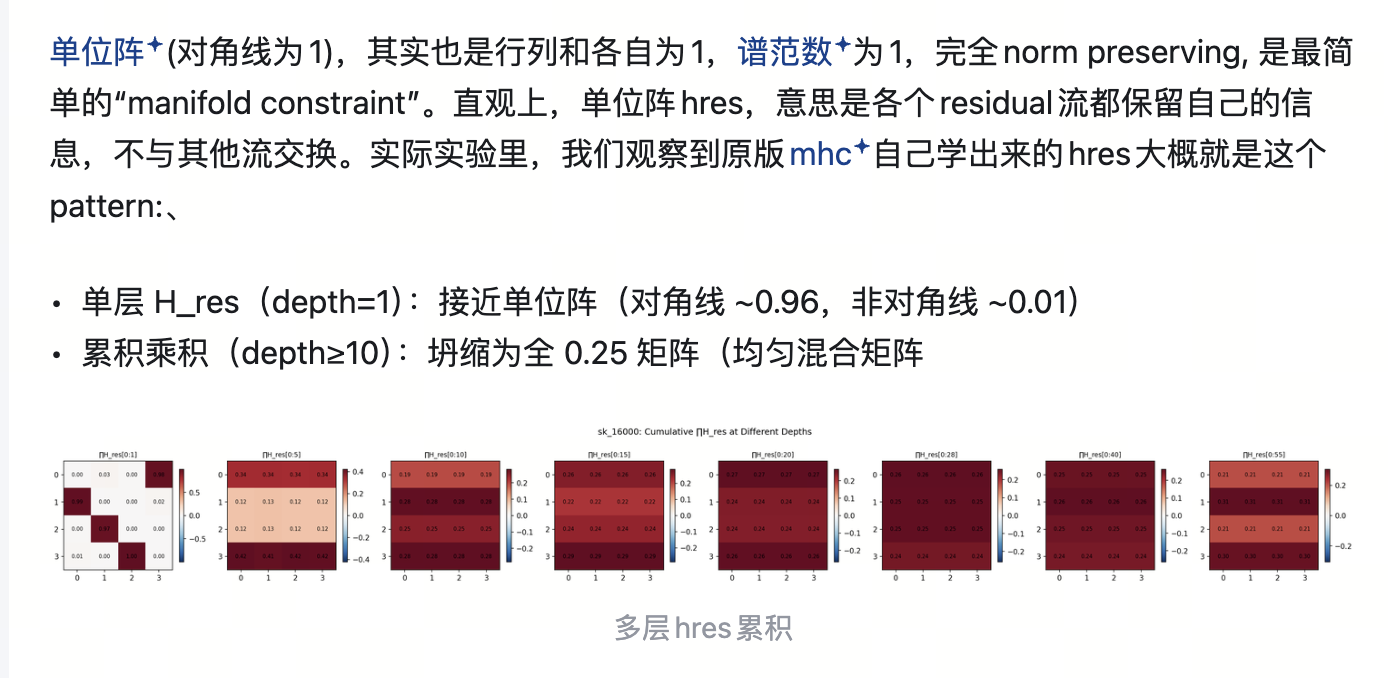
\includegraphics[width=0.68\linewidth,height=\textheight,keepaspectratio]{assets/ihc-observation.png}
\hfill\mbox{}

The screenshot describes identity as the simplest manifold constraint:
rows and columns sum to 1, the spectral norm is 1, and norms are fully
preserved. Each residual stream retains its own information without
exchanging it with others. In the original mHC experiments, a
single-layer residual mapping is near identity (diagonal about 0.96,
off-diagonal about 0.01), but products across 10 or more layers collapse
toward an all-0.25 averaging matrix. The bottom label reads ``cumulative
residual mappings across layers.''

The identity matrix is itself doubly stochastic, so it inherits the
benefits discussed under mHC. With hindsight, it may have a few
additional advantages:

\begin{enumerate}
\def\labelenumi{\arabic{enumi}.}
\item
  Numerical stability!
\item
  Each stream keeps its identity. The residual path can focus on
  preserving its own information, leaving reads, writes, and
  communication across streams to \(H^{\mathrm{pre}}\) and
  \(H^{\mathrm{post}}\).
\item
  \(H^{\mathrm{pre}}\) and \(H^{\mathrm{post}}\) no longer have to adapt
  to the reshuffling or mixing introduced by \(H^{\mathrm{res}}\).
\item
  No more SK, so infra finally gets a break from Sinkhorn-Knopp! Funny
  timing: as I write this, I'm watching the baffling ban/pick decisions
  of SK, the Wolves' coach in the KPL esports league\ldots{}
\end{enumerate}

\clearpage

\endgroup

\subsection{5. Gated Residual}\label{gated-residual}

Qwen3.8 Flash Next is my favorite paper of the year so far. Every design
choice deserves a close read.

The authors first expand the residual stream from \(1\) to \(n\), but
deliberately keep reading and writing simple: a static weighted sum for
reads, and writing to one branch at a time in rotation. This tests how
much ``just widening the residual stream'' can achieve. Widening alone
improves loss by 0.01, consistent with the earlier conclusion that wider
residual streams are central to HC.

The ablations reveal the following:

\begin{enumerate}
\def\labelenumi{\arabic{enumi}.}
\item
  \textbf{Simply widening the residual stream is already effective.}
\item
  \textbf{Data-dependent reads and writes still matter.} The improvement
  is especially clear on downstream benchmarks, more so than the loss
  alone suggests.
\item
  \textbf{Sigmoid works better than tanh for gating}, consistent with
  mHC's findings.
\item
  \textbf{Read granularity matters more than Write granularity.} Reads
  benefit from per-branch, per-channel control; a scalar per branch is
  enough for writes.
\item
  \textbf{Read/write operators should be predicted using information
  from all branches.} This works better than looking at only one branch
  or pooling first.
\item
  \textbf{Separate RMSNorm for each branch works better.}
\item
  \textbf{iHC gets it right: when reads and writes are strong enough,
  branch mixing through \(H^{\mathrm{res}}\) adds little.}
\end{enumerate}

GR Read therefore goes like this: independent RMSNorm for each branch →
concatenate all branches → low-rank MLP → sigmoid gates for each branch
and channel → average the gated branches to obtain the block input.

\subsection{6. Attention Residuals}\label{attention-residuals}

\begin{figure}
\centering
\pandocbounded{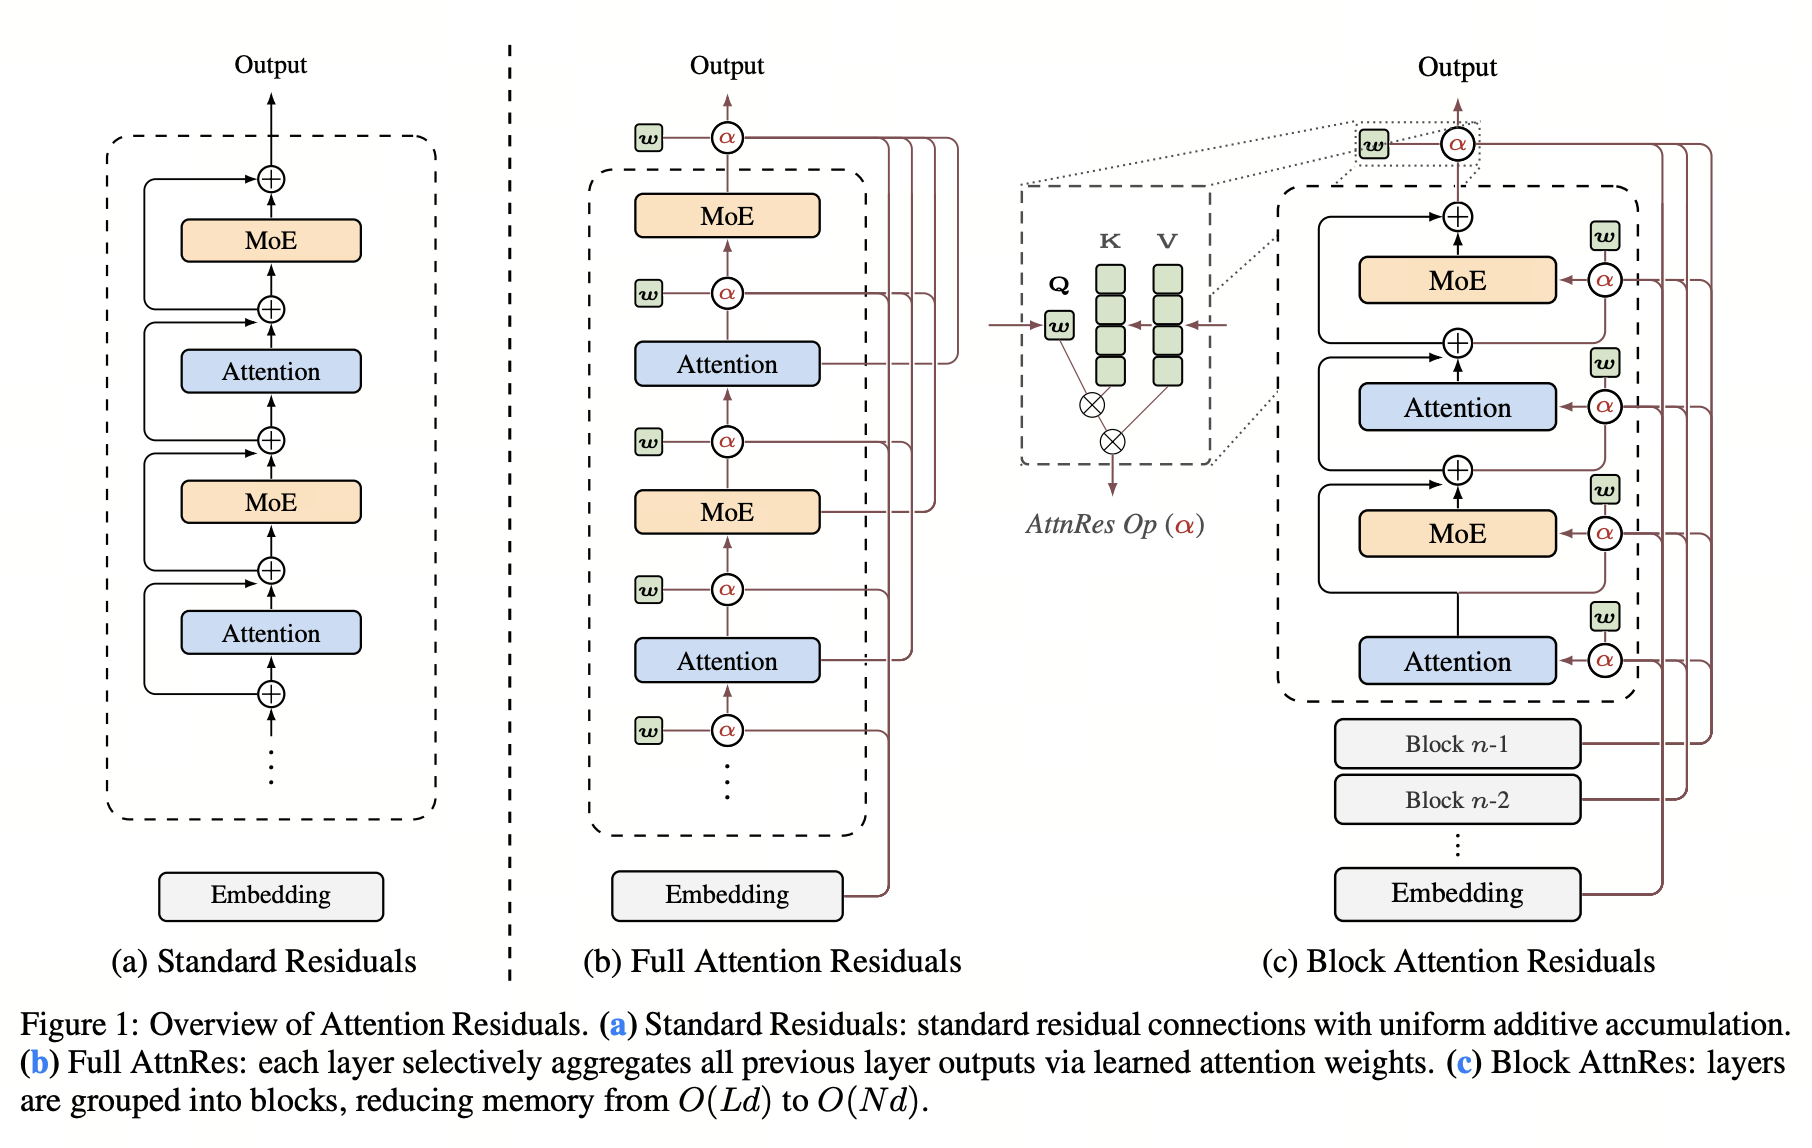
\includegraphics[keepaspectratio,alt={Attention Residuals architecture}]{assets/attnres.png}}
\caption{Attention Residuals architecture}
\end{figure}

An excellent paper. A vivid way to describe it is to rotate attention by
ninety degrees and apply it to the residual connections.

\subsubsection{Full AttnRes: Aggregating Earlier Representations Across
Depth}\label{full-attnres-aggregating-earlier-representations-across-depth}

In a standard Pre-Norm Transformer, the input to layer \(l\) can be
expanded as:

\[
h_l=h_1+\sum_{i=1}^{l-1}f_i(h_i).
\]

The embedding and all earlier sublayer outputs are accumulated into the
residual stream with a fixed weight of \(1\). AttnRes rewrites this as:

\[
h_l=\sum_{i=0}^{l-1}\alpha_{i\rightarrow l}v_i,
\qquad v_0=h_1,\quad v_i=f_i(h_i)\ (i\ge 1).
\]

The weights \(\alpha_{i\rightarrow l}\) are now learned dynamically
through softmax. Each target layer \(l\) introduces a learned
\(d\)-dimensional pseudo-query \(w_l\), with earlier layer outputs
serving as keys and values. Apply RMSNorm to the keys, then compute:

\[
s_{i,l}=w_l^\top\mathrm{RMSNorm}(v_i),
\qquad
\alpha_{i\rightarrow l}=\mathrm{softmax}_i(s_{i,l}).
\]

These weights are then used to aggregate earlier representations.
Although \(w_l\) itself does not depend on the token, \(v_i\) is
input-dependent, so each token still gets different routing across
layers. The authors initialize \(w_l\) to \(0\), giving every earlier
layer equal weight at the start of training, before the model gradually
learns selective connections.

Full AttnRes lets every layer attend directly to all preceding layers,
offering the finest-grained selection. But the memory and communication
demands are enormous; using it in an actual production model is not
realistic.

\subsubsection{Block AttnRes: Aggregating at the Block
Level}\label{block-attnres-aggregating-at-the-block-level}

Large models therefore mainly use Block AttnRes: group \(S\) consecutive
sublayers into a block, and retain ordinary residual accumulation within
that block:

\[
b_n=\sum_{j\in B_n}f_j(h_j).
\]

A new layer applies depth-wise attention only to completed historical
block representations \(b_0,\ldots,b_{n-1}\), with the partial sum of
the current block's already-computed sublayers included as another
candidate value.

This compresses ``retrieval by layer'' into ``retrieval by block.'' A
128-layer model, for instance, might maintain roughly 8 block sources
instead of 128 historical sources. Storage and communication costs fall
substantially, while preserving the key ability to actively look back at
information from distant depths.

On the infra side, the simple version---as for the deeper implementation
details, I don't fully understand them either!---is that Kimi mainly
uses three ideas: block grouping reduces the historical states that need
to be stored and accessed; input-independent queries allow inter-block
attention for a block to be precomputed in batches; and caching
historical block states trades memory for fewer repeated transfers in
the pipeline.

\subsection{7. xHC}\label{xhc}

\begin{figure}
\centering
\pandocbounded{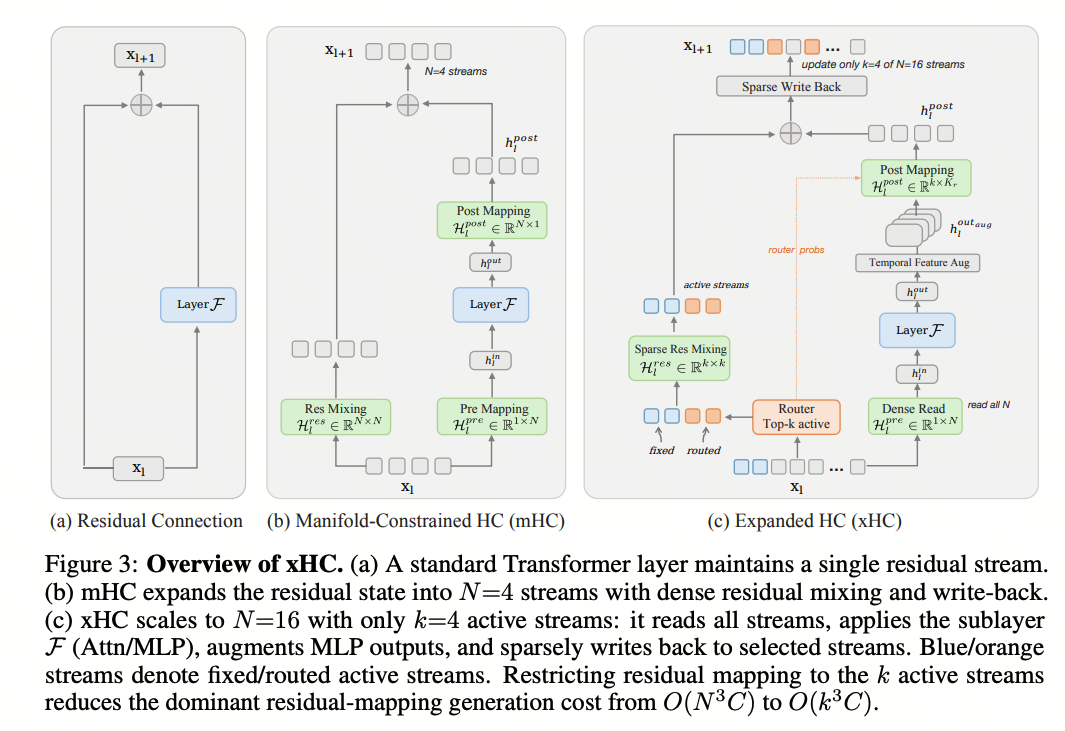
\includegraphics[keepaspectratio,alt={xHC architecture}]{assets/xhc.png}}
\caption{xHC architecture}
\end{figure}

This paper studies a problem left by HC/mHC: expanding the Transformer's
single residual stream into \(N\) parallel streams has mostly stopped at
\(N=4\). The authors identify two main barriers to increasing \(N\). The
first is an \textbf{information bottleneck}: each layer has only one
output to write back to \(N\) streams, so larger \(N\) makes it easy for
the streams to learn redundant histories. The second is a \textbf{cost
bottleneck}: mHC dynamically generates an \(N\times N\) residual mixing
matrix from an \(NC\)-dimensional state, giving the corresponding
projection a complexity of \(O(N^3C)\).

xHC tackles both. On the information side, it applies three causal
depthwise 1D convolutions after the MLP output, with kernel sizes
4/8/12. The current output and local context at different time scales
form four write-back components, with Gram-Schmidt reducing their
collinearity. On the computation side, it uses \textbf{dense read +
sparse write}: there are \(N=16\) residual streams, but each layer
activates only \(k=4\) for residual mixing and write-back. Two are
always active; a router dynamically selects the other two. The layer
input still reads densely from all 16 streams. This retains the
persistent state / memory of 16 streams while reducing the most
expensive residual-mapping component from \(O(N^3C)\) to \(O(k^3C)\).

\subsection{8. VWN}\label{vwn}

VWN is a paper I keep thinking of as an overlooked gem. It is a really,
really, really good paper, yet it has only two citations as I write
this. It starts from a different motivation:

\textbf{Increasing a Transformer's hidden width often improves its
representational capacity, but Attention/FFN computation and parameter
counts grow roughly quadratically with width. MoE can expand FFN
capacity cheaply, yet it leaves the representational bottleneck of the
backbone hidden dimension unresolved.} How can we make the model wider
without increasing computation too much?

\begin{figure}
\centering
\pandocbounded{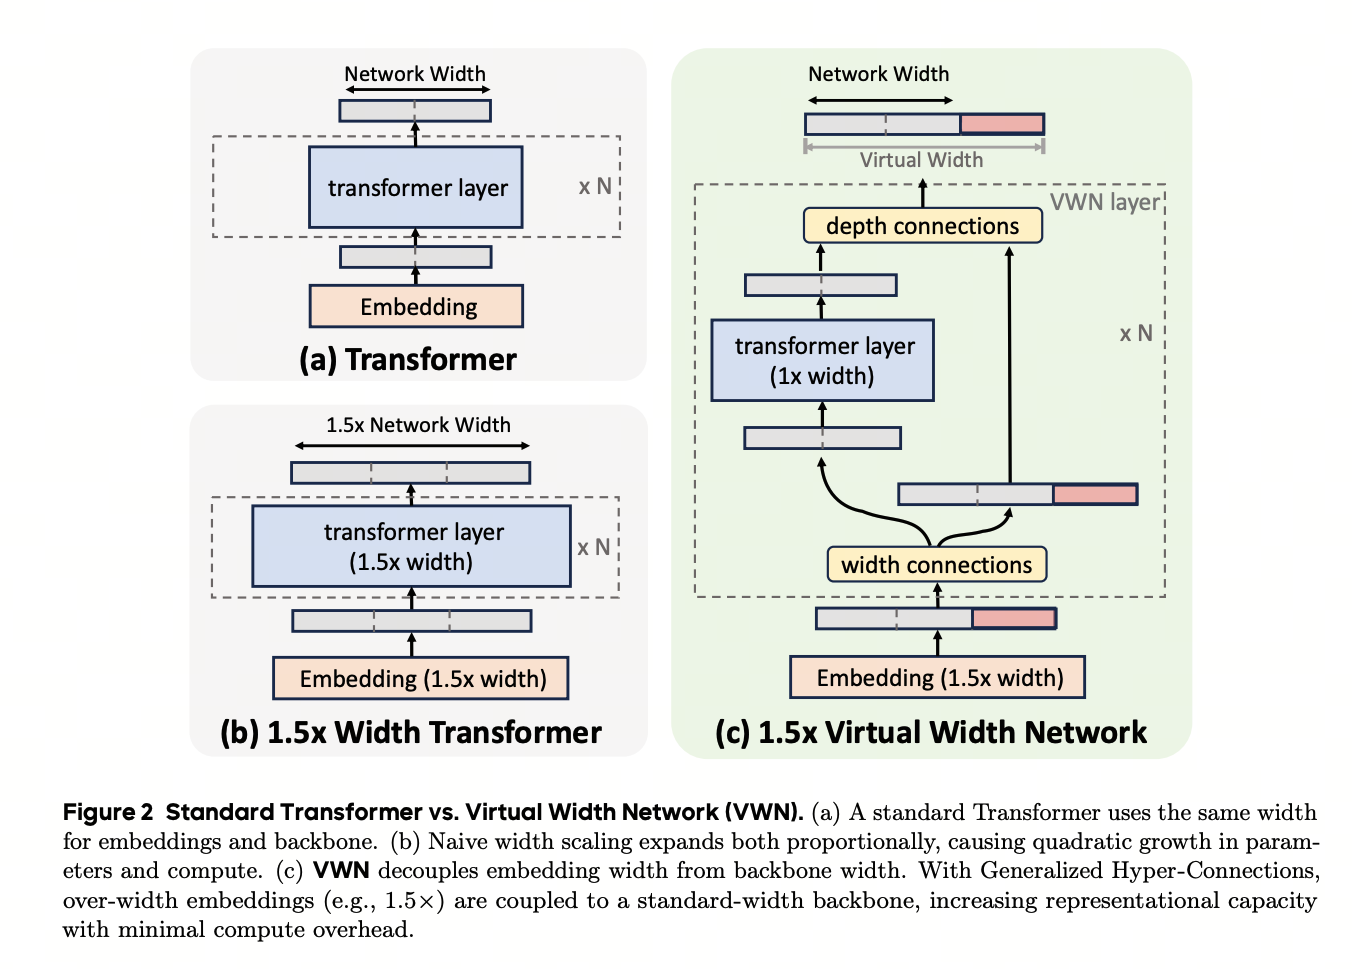
\includegraphics[keepaspectratio,alt={VWN overview: representation width and computation width}]{assets/vwn-width.png}}
\caption{VWN overview: representation width and computation width}
\end{figure}

VWN decouples ``representation width'' from ``actual computation
width.'' Tokens and hidden states carried across layers maintain an
\(rD\)-dimensional \textbf{over-width representation}. Before each
Attention/FFN computation, Generalized Hyper-Connections (GHC)
dynamically compress this to \(D\) dimensions; after computation, the
output is written back to the wide state. The expensive Transformer
backbone therefore remains \(D\)-wide.

\begin{figure}
\centering
\pandocbounded{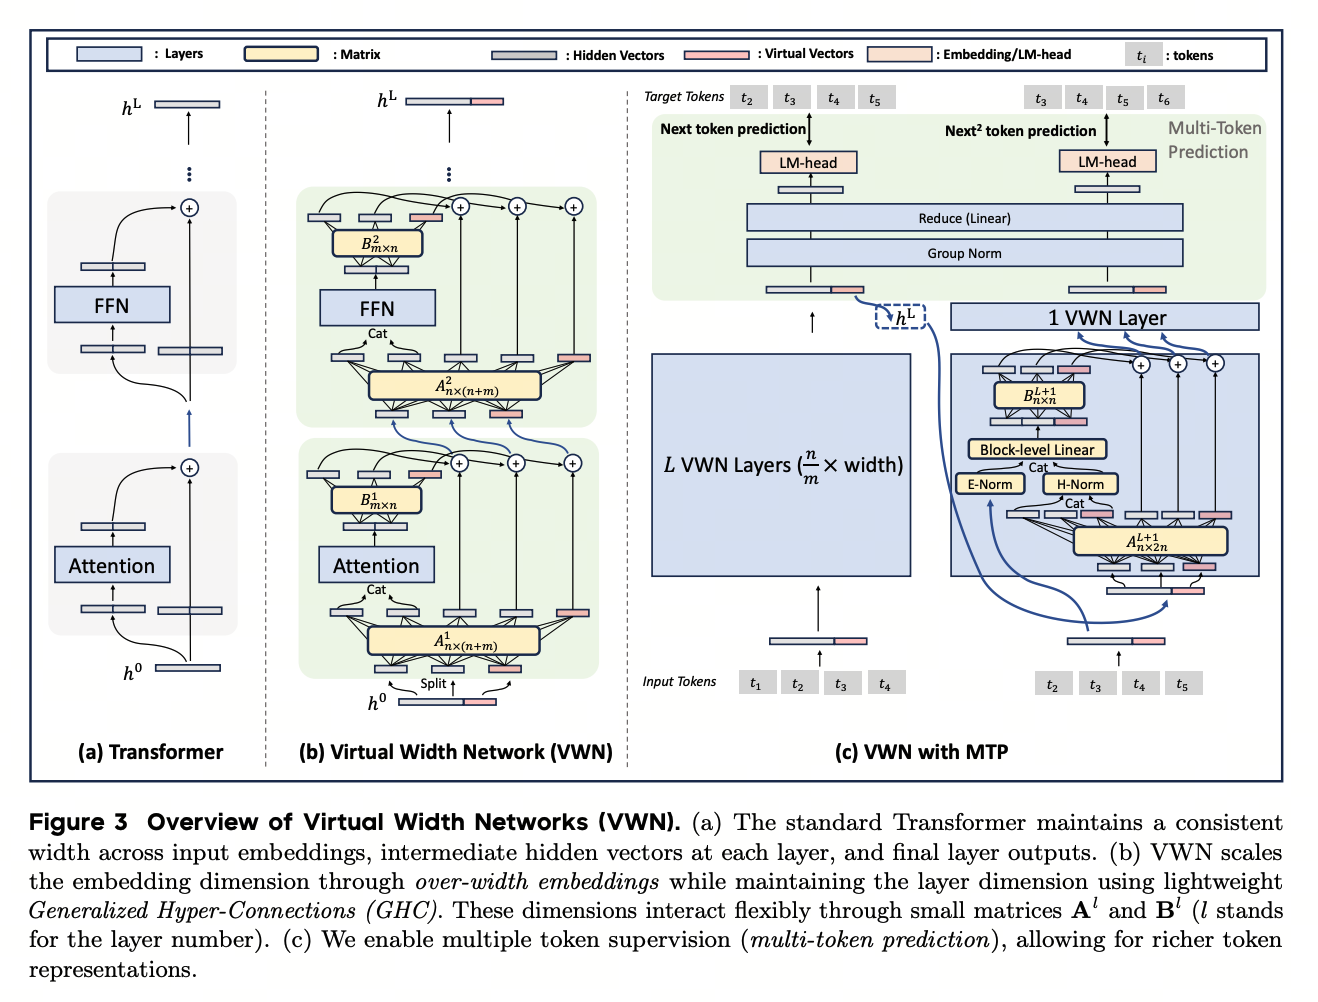
\includegraphics[keepaspectratio,alt={VWN architecture and its combination with MTP}]{assets/vwn-architecture.png}}
\caption{VWN architecture and its combination with MTP}
\end{figure}

GHC also divides the wide state into multiple slots, using learned
\(A\)/\(B\) routing matrices to carry, mix, and update information
across layers. At the output, it reduces the state back to \(D\)
dimensions.

The paper further combines VWN with Multi-Token Prediction (MTP), aiming
to use denser prediction supervision to make full use of the additional
representational freedom.

\end{document}
